\section{Interpreting the Data}
\label{sec:datainterpret}


GAStech has given a large quantity of data  in order to identify unusual patterns of behaviour that may be related to the missing staff. This consists of various information about the different employees, including GPS tracking data, their credit card usage and loyalty card usage.

\subsection{Data Provided}
\label{sec:dataprovided}

The Car ID Assignment and Job Role data consists of the first and last names of the employees whose vehicles are tracked, and also their department, their employment title and an ID number associated with their vehicle. \\

\noindent However there are nine employees, all of whom are truck drivers, who do not have a car ID assigned to them. As a result it is not clear which route belongs to which truck driver, meaning that there is some uncertainty within the data. This problem is approached in section~\ref{sec:completedata}. \\

\noindent GPS tracking data is also supplied for 40 different company vehicles.  This data consists of latitude, longitude, a timestamp, and a vehicle ID number to link these vehicles back to people. It is the largest dataset supplied; it holds 14 days worth of GPS Tracking data for each ID. It allows the exact location of each vehicle supplied by the company to be known whenever the vehicle is moving, and also at what time this vehicle is moving. \\

\noindent The credit card data includes a timestamp to show the time of the transaction and establishment names to show where the transaction takes place. It also states how much was spent and who is using the credit card. Unlike the GPS data, this set gives a name as opposed to an ID number, which means that in order to link this data with the GPS data, the car ID assignment data must be cross-referenced and transactions must be matched to each employee. \\

 It is necessary to complete the data to allow a thorough analysis of the employees’ behaviours as the data provided is incomplete,. The locations of the establishments where credit cards and loyalty cards are used are unknown, as is the exact Identification of the truck drivers. Additionally the credit card data, loyalty card data and tracking data is of different resolutions. The tracking data gives the time to the nearest second, the credit card data gives the time of the transaction to the nearest minute, while the loyalty card data only gives the day of the transaction. The loyalty card data gives no assistance when finding the exact location of the establishments due to the low resolution. \\

\subsection{Initial Analysis of the Data}
\label{sec:initialanalysis}

Figure~\ref{fig:gpsdata} shows all of the GPS data for all employees with a company vehicle. There are some denser areas, near the centre of the graph, from this it can be deduced that people tend to make the same kind of journeys each day. There are also some journeys which are singular, and these are shown on the graph by the areas with sparse data. These are the journeys that need to be sought out as they are more likely to be the anomalies. \\

\begin{figure}[!ht]
\centering
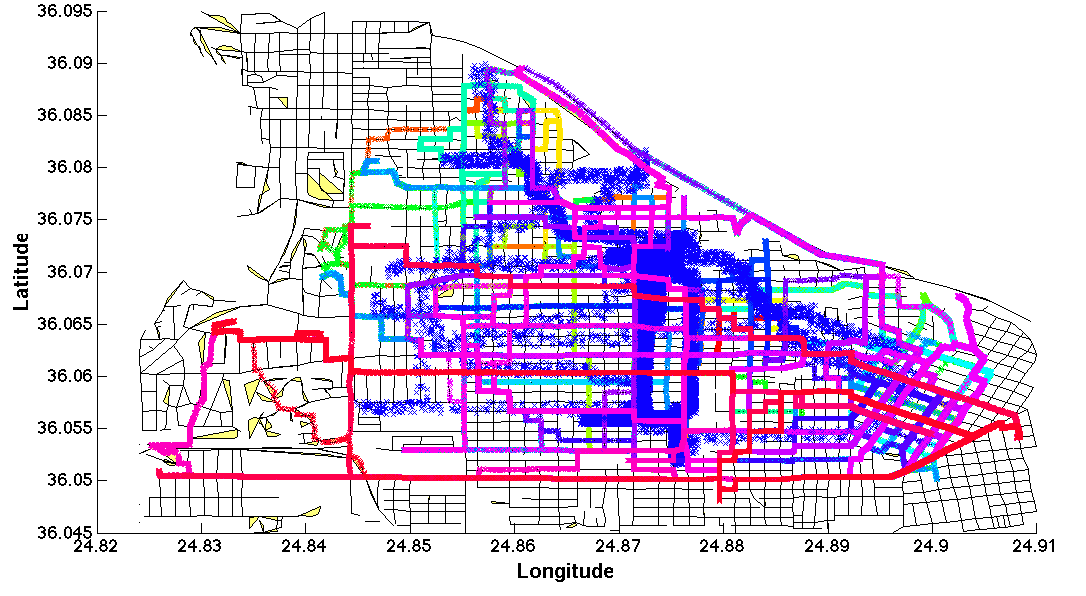
\includegraphics[width=0.9\textwidth]{gpsdata.png}
\caption{\label{fig:gpsdata}A plot showing all GPS data provided.}
\end{figure}


\noindent  Figure~\ref{fig:spending} shows the spending patterns of the employees. The cluster of lines towards the bottom of the graph shows that most employees have a similar spending pattern. There are ten employees who spend much more. The majority of these outliers are truck drivers, who spend a lot of money on fuel, however there is one outlier, Lucas Alcazar who is an IT Helpdesk assistant who spent a total of 11,454.00 which is unusually high in comparison to other employees with the same job. \\
\begin{figure}[!ht]
\centering
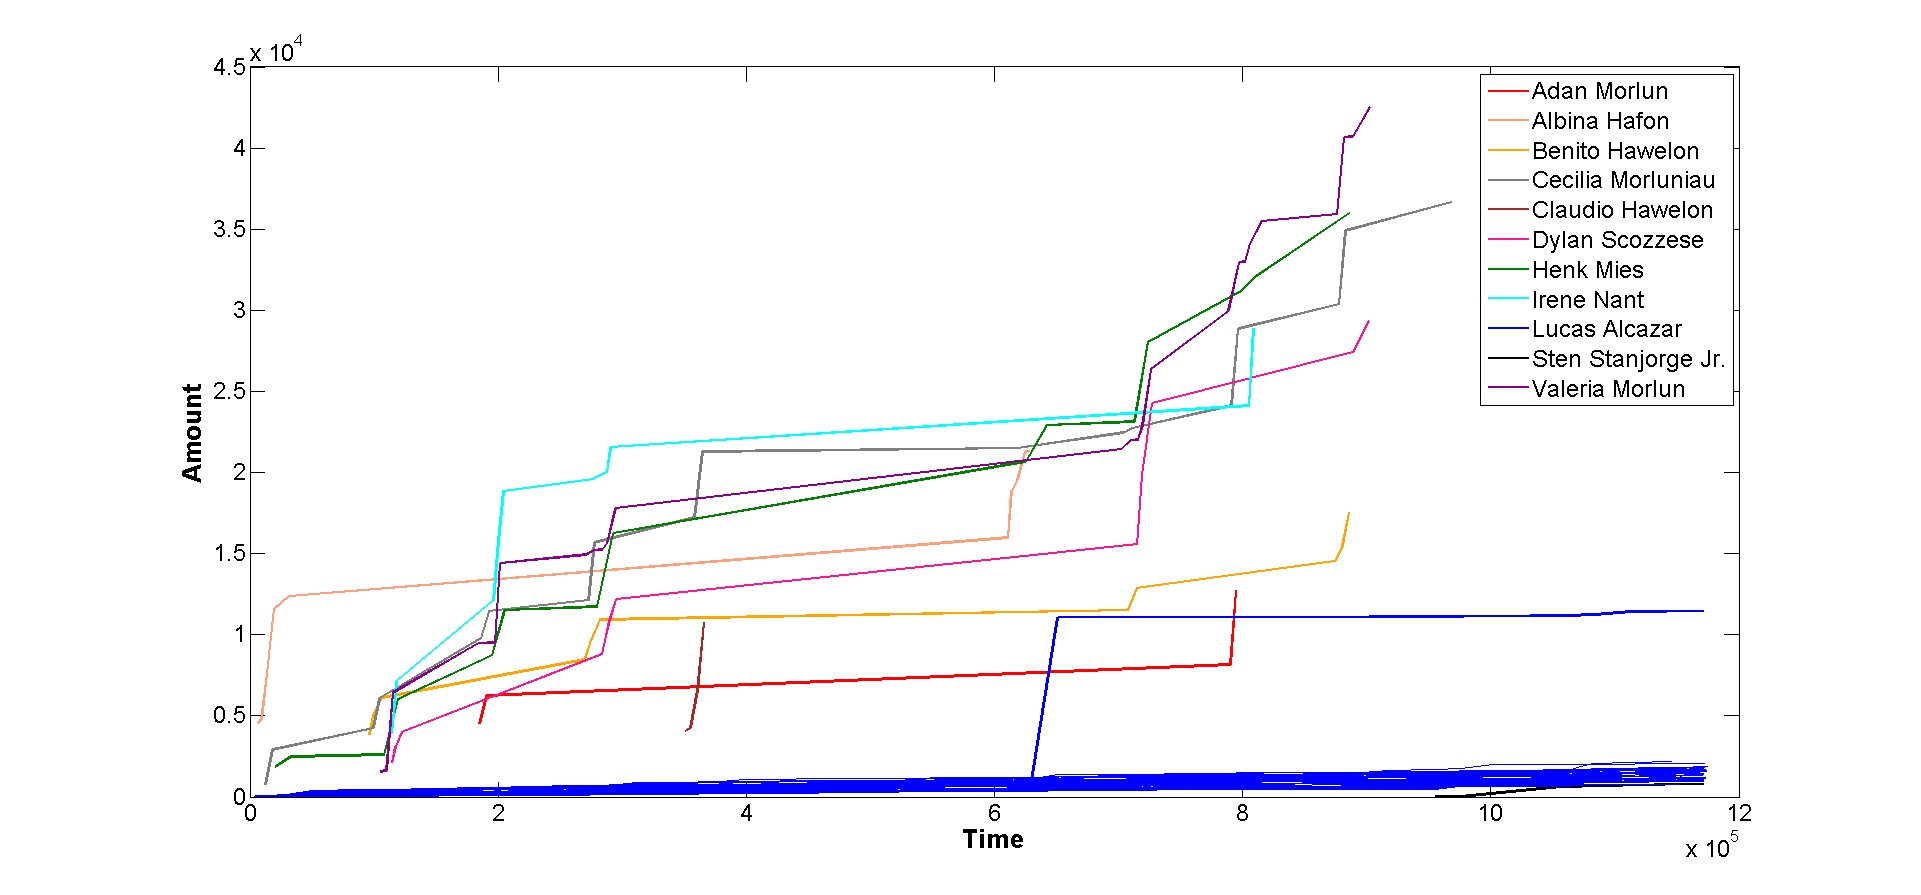
\includegraphics[width=1.0\textwidth]{spending.png}
\caption{\label{fig:spending}Total amount spent on each person's credit card.}
\end{figure}



